\section{Introdução}
\label{sec:introducao}

O objeto deste trabalho é um software comercial de neurofeedback que executa inteiramente na máquina do cliente. Construído em Avalonia sobre .NET~10, no padrão MVVM, ele lê o sinal de eletroencefalografia (EEG) de um sensor BrainBit Flex~4 por meio do SDK do fabricante, processa esse sinal com um algoritmo proprietário e devolve ao paciente o feedback do treino. É distribuído por instalador, sem atualização automática, e chegou ao início do projeto sem nenhum controle de segurança: um \enquote{white canvas}. O nome do produto e o da empresa ficam fora deste relatório e do repositório, que é público.

Quando um software roda por completo no ambiente do usuário, o fornecedor perde o controle sobre ele: quem possui a máquina pode inspecionar, copiar e modificar o programa à vontade. É o modelo de atacante conhecido como Man-At-The-End (MATE), em que o adversário controla o próprio ambiente de execução \parencite{collberg2009}, situação bem diferente daquela em que o atacante está apenas na rede entre duas partes. Desse cenário derivam as duas dores que o projeto se propôs a tratar, ambas com impacto direto no negócio: o uso do software sem licença válida (pirataria) e a recuperação do algoritmo proprietário de processamento de sinal a partir do binário (roubo de propriedade intelectual).

Em vez de tratar segurança como uma funcionalidade acrescentada no fim, o software foi conduzido por um processo iterativo de endurecimento, estruturado como Test-Driven Security \parencite{vehent2018} com purple teaming. Um time azul (blue team) construiu cinco versões do aplicativo, da v0 à v4, com controles crescentes; um time vermelho (red team) atacou cada uma em caixa preta; e cada ataque bem-sucedido virou um teste de regressão que roda na esteira de integração contínua a cada mudança. Cada tentativa, inclusive as que falharam, teve o custo medido em minutos.

A premissa que orienta o trabalho é honesta: em um cenário MATE não existe proteção absoluta. O objetivo viável, e a métrica do projeto, é elevar o custo do ataque acima do valor do ativo protegido, na linha do projeto ASPIRE \parencite{aspire}. Por isso a contribuição pretendida não é um software definitivamente blindado, o que seria inviável, e sim a demonstração documentada de um processo replicável de endurecimento, acompanhada da medição de quanto cada iteração encarece o ataque. Esse processo está inteiro no repositório do projeto \parencite{repo}, que funciona como modelo para reuso: modelo de ameaças, casos de abuso, árvores de ataque, matriz de rastreabilidade, plano das iterações, guia do red team, uma nota por build, o registro de custo, a suíte de testes de ataque e a esteira.

No Cyber Security Body of Knowledge (CyBOK) \parencite{cybok2021}, o trabalho se situa na categoria de Segurança de Software e Plataforma, na área de conhecimento de Ciclo de Vida de Desenvolvimento Seguro, com apoio da área de Segurança de Software. A Figura~\ref{fig:infografico} resume o projeto.

\begin{figure}[htbp]
\centering
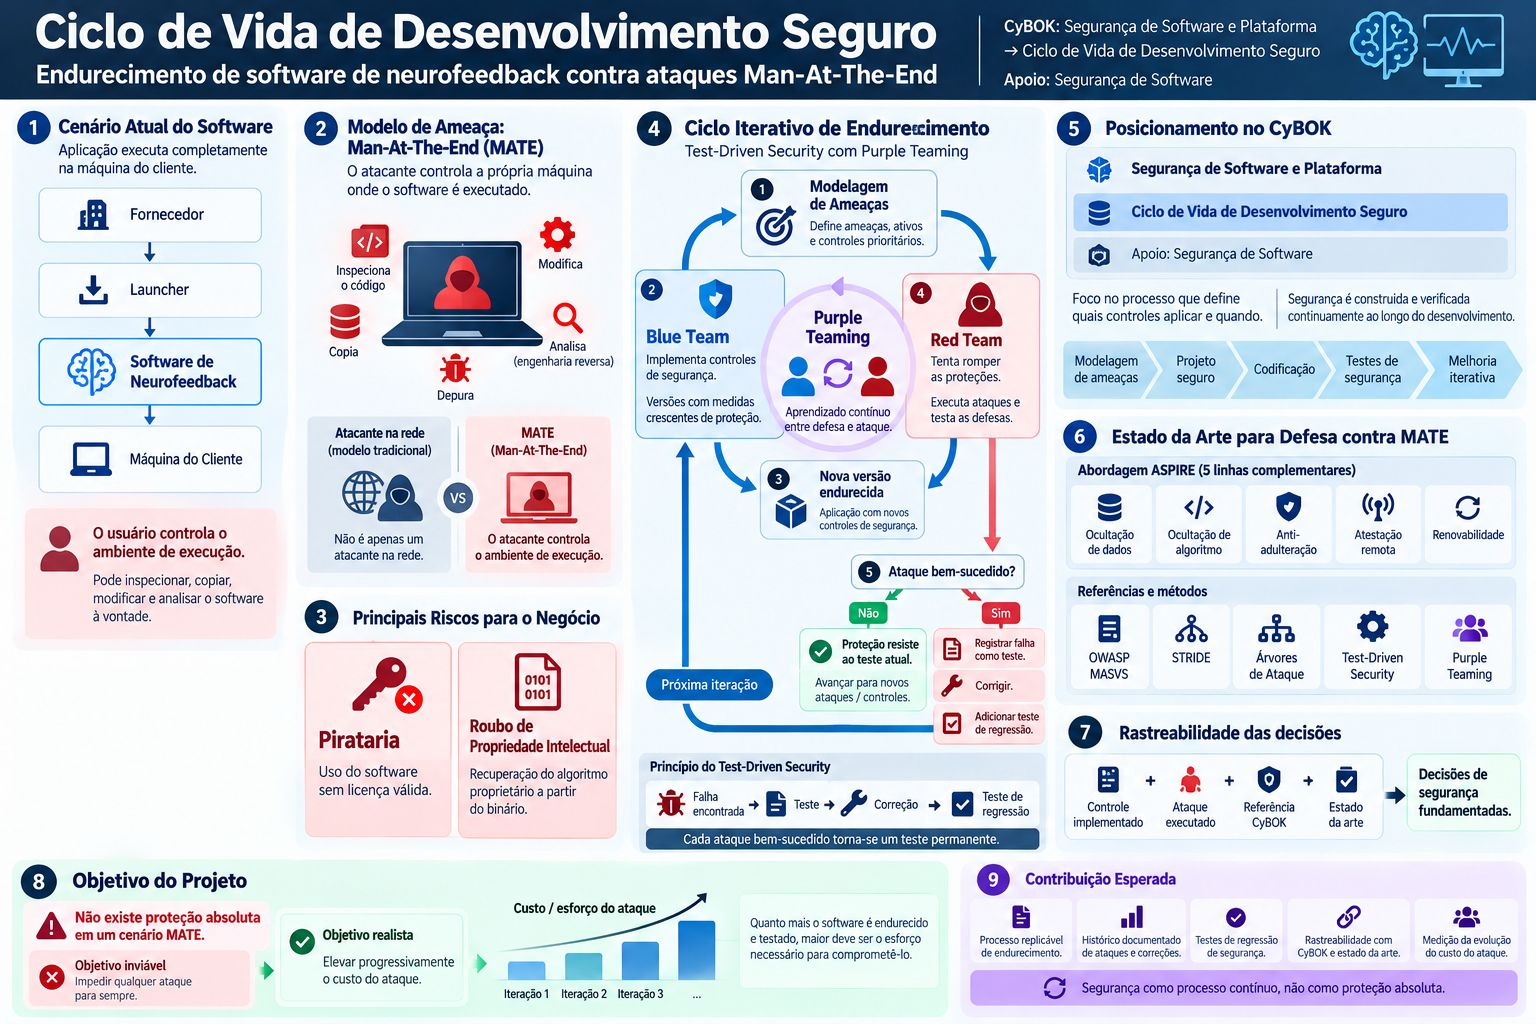
\includegraphics[width=\textwidth]{infografico.jpg}
\caption{Visão geral do projeto: cenário, modelo de ameaça, riscos, ciclo iterativo red e blue, posicionamento no CyBOK, estado da arte e objetivo.}
\label{fig:infografico}
\end{figure}

O resultado medido ao longo das cinco builds, em resumo, foi o seguinte. Para a pirataria, o ataque mais barato que funcionava custou 5 minutos na v0 e deixou de existir na v3 e na v4: nenhum caminho conhecido funcionou, e o red team gastou até 45 minutos sem sucesso numa mesma build. Para o roubo do algoritmo, o custo do caminho completo mais barato dobrou, de 5 para 10 minutos, mas a árvore de ataque seguiu aberta, porque o algoritmo continua executando na máquina do atacante. Em uma frase: dá para tornar a pirataria cara demais para valer a pena; o algoritmo dá para encarecer, mas não para esconder.

O restante do relatório percorre os artefatos do repositório na ordem em que foram produzidos. A Seção~\ref{sec:fundamentacao} apresenta a fundamentação e o estado da arte, e a Seção~\ref{sec:objeto} descreve o aplicativo e o mock usado no lugar dele. As Seções~\ref{sec:ameacas} a~\ref{sec:arvores} cobrem a modelagem de ameaças, os casos de abuso e as árvores de ataque. A Seção~\ref{sec:processo} detalha o processo, a suíte de testes e a esteira, e a Seção~\ref{sec:rastreabilidade}, a matriz de rastreabilidade. A Seção~\ref{sec:iteracoes} narra as cinco iterações, a Seção~\ref{sec:resultados} reúne os resultados, a Seção~\ref{sec:discussao} os discute e a Seção~\ref{sec:conclusao} conclui. O Apêndice~\ref{ap:custos} transcreve o registro completo de custo.
